\newpage
`
\newpage
\begin{appendices}
\section{Design Document} \label{App:design-document}

\subsection{  Content Based Access Control for Swift Storage }
Our proof of concept prototype works only on JSON formatted data stored in swift.

\subsubsection{ Usecase}
Alice has a  data file ('data.json') stored in Swift. With  Swift-ACL she can specify who can or cannot access the file, but she also want to define who can access how much content of the file. In other words,  besides using ACL, she wants to specify access control on the content level of the file.  So, she  attaches a  policy ('policy.json')  with the file and wants that all the access request to the file would honor the policy associated with the file.

\subsubsection{Design Details}
As mentioned in the usecase, we would attach a policy with the object available in  Swift storage. The policy  would specify who can or cannot access which part of the associated document. The policy would be stored as metadata associated with the object. In the object server, when the object is  retrieved, we also retrieve the policy. In our access control module we feed both the requested object and the policy. The response from the access control module is the partial content of the object – the requester is allowed to access. Figure \ref{fig:swift-content-filter} shows the design diagram for our case.

\subsubsection{Proposed Changes}
The proposed changes are only at the object server middleware.

\begin{itemize}

\item \emph{Policy file}: We would specify syntax for the policy that Alice can use. The policy would be stored as metadata associated with the object.
\item \emph{A/C Module}: The Access Control module takes a input file in JSON format and  policy for it along with the credential of the requested user. The result from the A/C module is the partial content of the object – the requester is allowed to see.

\end{itemize}

\begin{figure*}[t]
\centering
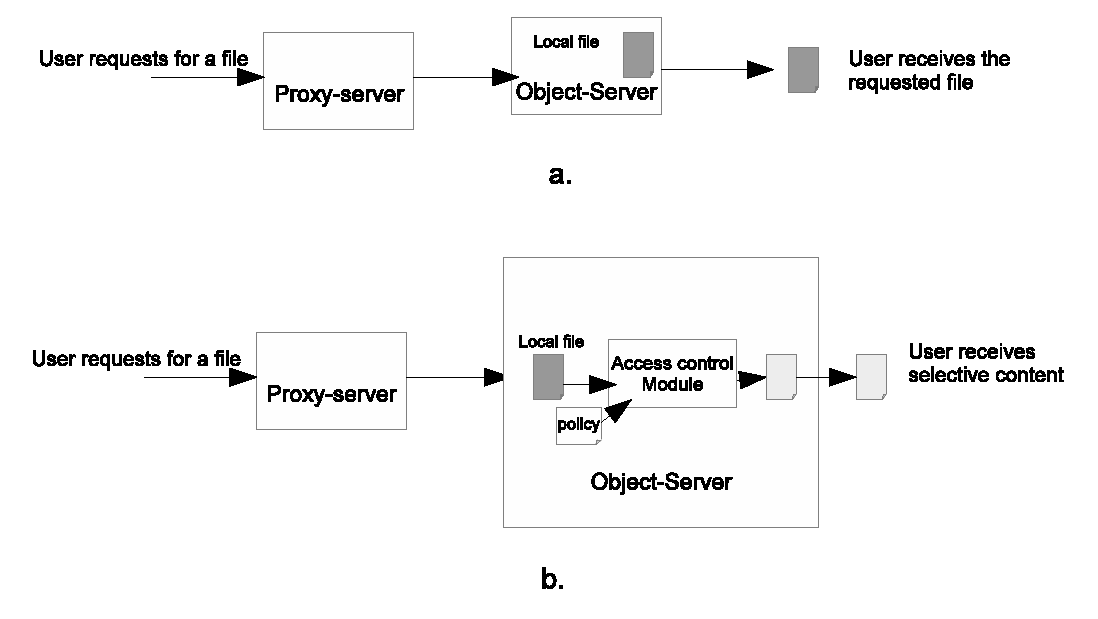
\includegraphics {eps/swift-content-filter}
\caption{a. Evaluation of the GET Request for Swift, b.   Evaluation of the GET Request for  Swift with Proposed Content Filter.}
\label{fig:swift-content-filter}
\end{figure*}

\subsection{ ZeroVM enabled Content Based Access Control for Swift Storage} 

\subsubsection{ Usecase}
ZeroVM enables a user to run arbitrary application on Swift data located inside Swift storage by virtue of a ZeroVM Application. Bob wants to run a ZeroVM application with his own executable (A python script for example) on Alices  protected data object ('data.json'). But this time Alice does not worry because she knows a ZeroVM developer is working on Swift Zerocloud midleware that would restrict any arbitrary access on her data object by ZeroVM application owned by other users.

With our proposed design, we would restrict any zerovm application to respect policy set by the owner of a swift data object.

This use case differs from the former case  in the sense that in the former case, a user is accessing a Swift object, and in the later case, an application is accessing the object for purpose of arbitrary processing. While in the former case, data object leaves Swift storage, in the later case data object does not actually leave Swift storage.

\subsubsection{Design Details} 
In the existing approach, the manifest file of a ZeroVM application contain list of input files, output files and image files possibly containing user application.  On receiving exection request, a ZeroVM is launched inside the object server and the user application can arbitrarily access the full content of these files. 

In our proposed architecture, we let not allow full content of the Swift objects listed as input to be visible to the user application. In order to achieve this, we introduce the concept of Query. In this case,  when the ZeroVM manifest contains a Swift object as input, it also contains predefined queries on that object.  In the final manifest for the ZeroVM, the input object is not attached as a channel, instead the temporary files containing the output of the queries are attached as input channels. This is how, we would hide the visibility of the full content of the Swift objects as input.  In processing the queries against a input Swift object, we apply the policy associated with the  object.

 To make our implementation simple, we would use a JSONPath as the a query. While Figure \ref{fig:abstracted-zapp} shows the abstracted view of existing ZeroVM application, our proposed design detail is shown in Figure \ref{fig:proposed-zapp}

\begin{figure*}[t]
\centering
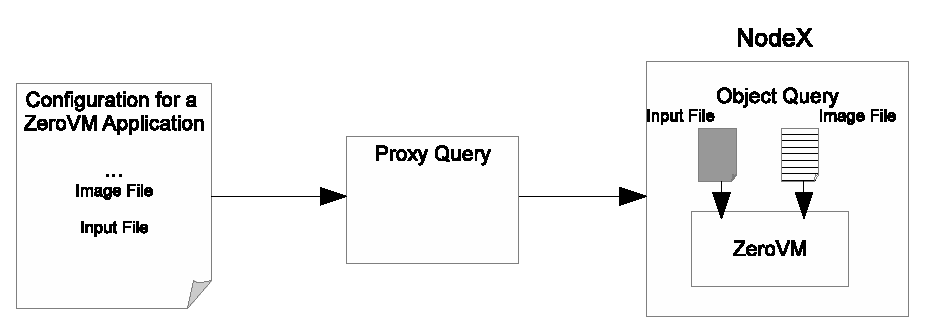
\includegraphics {eps/abstracted-zapp}
\caption{Abstracted Design for Existing ZeroVM Application .}
\label{fig:abstracted-zapp}
\end{figure*}

\begin{figure*}[t]
\centering
\includegraphics {eps/proposed-zapp}
\caption{Design for ZeroVM Application With Proposed Content Filter.}
\label{fig:proposed-zapp}
\end{figure*}

\subsubsection{Proposed Changes}
The proposed changes are made  at the manifest of the ZeroVM application along with at the object query middleware of the zerocloud.

\begin{itemize}

\item \emph{Add query section in the manifest of ZeroVM application}:  

\item \emph{Query Engine}: The query engine takes a query which is JSONPath in our case, and execute the query against the Swift object. The output of these queries are being saved in temporary files and these file descriptors are feed into the launching ZeroVM as input channels.

\item \emph{A/C Module}: We develop an  access control module for JSON document which takes a JSON document, a policy file stating which part of the document is accessible by which user, and a set of queries. This module with the help of Query Engine module generates output for these queries.

\end{itemize}

\end{appendices}
